%!TEX encoding = UTF-8 Unicode
% !TeX spellcheck = en_GB

%%%%%%%%%%%%%%%%%%%%%%%%%%%%%%%%%%%%%%
\chapter{ Overview of Higgs pair production at colliders }\label{chap:overviewDiHiggs}
%%%%%%%%%%%%%%%%%%%%%%%%%%%%%%%%%%%%%%
The determination of the shape of the Higgs potential is an essential part of the LHC physics programme. Unlike the determination  of most properties of the Higgs and its couplings to heavy particles, the light Yukawa and Higgs-self couplings  are exceptionally hard to probe.  This is particularly evident from the conclusion of ~\autoref{chap:4topSingleHiggs}. When we have seen that the effectiveness of the utilisation of single Higgs signals in order to probe the Higgs trilinear coupling is challenged with the fact that other weakly constrained operators also affect these signals. Thus, Higgs pair production remains as thee only direct way to access this elusive interaction. \\ The production of Higgs in pairs has roughly $ 10^{-4} $ the signal of producing a single Higgs at the LHC. The  Higgs pair production with Higgs pair decays considered have a cross-section of $ \sim 1 \si{\femtobarn}$, in the SM. This would make it inaccessible from Run-II or Run-III data, but should be accessed using the whole luminosity of the HL-LHC ~\cite{Apollinari:2015bam,ATL-PHYS-PUB-2018-053,Cepeda:2019klc}. As for the quartic coupling, which would require NLO corrections to Higgs pair, which are currently unknown, or triple Higgs production, both of which are beyond the sensitivity of the LHC~\cite{Plehn:2005nk}. The measurement potentials for the light Yukawa couplings shall be discussed in the Next chapter.   The main advantages for Higgs pair production in determining the Higgs trilinear self-coupling comes from the dependence of the cross-section of $\lambda_3$ at the LO level, as well as the fact that the rest of SMEFT operators entering in this process~(see eq~\eqref{HH-smeft}) can be strongly constraint from other processes, breaking any potential correlations that might appear between them and the trilinear coupling using only di-Higgs data. However, the inclusion of light quark Yukawa couplings modifiers e.g.$ C_{u\phi}$ and $C_{d \phi}$ would complicate things as we shall see in~\autoref{chap:MLLightYuk}. \\
This chapter will start by reviewing the theoretical status of the dominant process for Higgs pair production, the gluon fusion, in~\autoref{ggFhh}. Then, the other subdominant channels will be briefly reviewed in~\autoref{otherhh}. I will afterwards overview the experimental efforts in probing this rare yet fascinating processes in~\autoref{exphh}. Finally, I will present  in~\autoref{summtrilinear} a summery of the trilinear Higgs-self coupling constraints. 
%%%%%%%%%%%%%%%%%%%%%%%%%%%%%%%%%%
\section{Higgs pair production by gluon fusion \label{ggFhh}  }
%%%%%%%%%%%%%%%%%%%%%%%%%%%%%%%%%%
The dominant process for Higgs pair production at the LHC~(and hadron colliders in general) is the gluon gluon fusion~(ggF) via a heavy quark loop~$Q$, mainly the top and beauty quark, with the latter contributing only to about~$1\%$, as shown in~\autoref{fig_ggf_sm}.
%
\begin{figure}[!htpb]
	\centering
	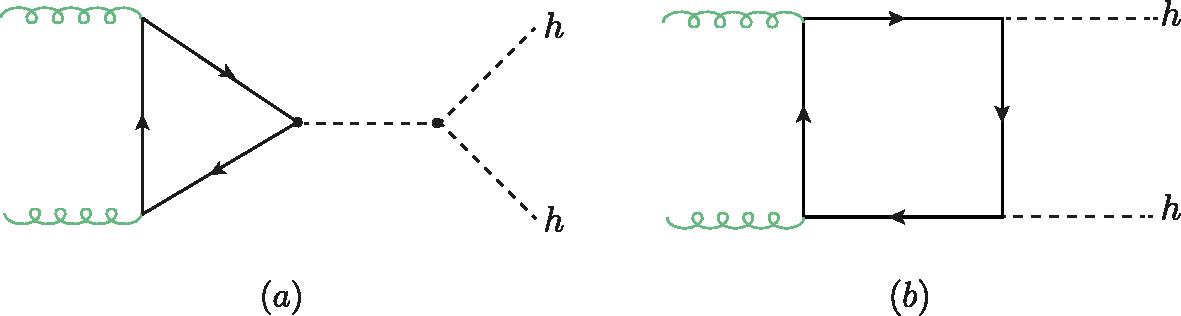
\includegraphics[width = 0.8\textwidth]{./figures/di-higgs-LO-SM}
	\caption{Feynman diagrams for the ggF process of Higgs pair production in the SM.} 
	\label{fig_ggf_sm}
\end{figure}
%
This process is well-studied at leading order~(LO) analytically~\cite{EBOLI1987269,GLOVER1988282,DICUS1988457,Plehn:1996wb}.  The higher order computations are significantly more complicated to preform compared to the gluon fusion production of a single Higgs. This is due to the fact that multi-scale amplitudes at two-loops (and more) cannot be always computed analytically using the current computational techniques.  The first attempt to compute the NLO corrections to di-Higgs were via the infinite top limit (HTL/LME)  approximation~\cite{Dawson:1998py, Altenkamp:2012sx,Grigo:2014jma} and implemented in~\texttt{HPAIR}. These corrections were found to be large, with a K-factor of $ \sim 2$.  This prompted more calculations with inclusion of top mass effects~\cite{deFlorian:2013uza,Grigo:2013rya,Maltoni:2014eza,Grigo:2015dia,Degrassi:2016vss}, which improved the stability of the LME expansion as well as corrected the cross-section by $\sim 10\%$. In addition, the threshold resummation effects of the LME has been included in \cite{Shao:2013bz}. This approach, however, is not sufficient to produce corrections to the differential cross-section, as the LME fails for $m_{hh}^2/4m_t^2 \lesssim 1$. Using numerical evaluation of the two-loop integrals, it is possible to obtain exact results with full top mass dependence, see refs.~\cite{Borowka:2016ypz,Borowka:2016ehy,Baglio:2018lrj}. But this comes at the cost of computational power required to evaluate the cross-section.  Hence, approximation methods were imperative in obtaining more flexible results for use at simulations and BSM Higgs pair production predictions.  These approximations methods are analogous, and sometimes connected  to the ones used for $Zh$ production discussed in~\autoref{chap:hz}. This includes, small final particle transverse momentum ~\cite{Bonciani:2018omm}, and high energy~(HE) expansions~\cite{Davies:2018ood,Davies:2018qvx}. In addition to a method developed in refs. ~\cite{Xu:2018eos,Wang:2020nnr} which considers both $\hat s , \hat t$ and $m_t$ as large quantities while keeping the Higgs mass as small one. This method has a wide coverage of the $m_{hh}$ spectrum.  The use of Pad\'e approximation to improve the $\pt$--expanded amplitude coverage as well as to obtain a description for the three-loop~(NNLO) form factors was demonstrated in~\cite{Davies:2019nhm}. The NNLO cross section with top mass effects has been computed numerically in~\cite{Grazzini:2018bsd} and also at differential level~\cite{deFlorian:2016uhr}, and analytically only in the LME~\cite{deFlorian:2013jea}. Also, NLO+ NNL analytic results have been obtained by~\cite{deFlorian:2015moa}. Parton shower matching for NLO Higgs pair production has been computed  in~\cite{Jones:2017giv,Heinrich:2019bkc}, which was essential for the \texttt{POWHEG} implementation for di-Higgs, with NLO corrections computed from a grid has been made available by ~\cite{Heinrich:2017kxx,Heinrich:2019bkc,Heinrich:2020ckp}. \autoref{dihiggs-gridplot} shows the Higgs pair virtual partonic cross-section defined in~eq.\eqref{eq:deltasigma} vs the  $\pt$ and HE expansions bridged using Pad\'e  approximants~\la{add ref}. \\
%
Moreover, the NLO Higgs pair production with SMEFT operators is available in \texttt{SMEFTatNLO} mode~\cite{Degrande:2020evl} for ~\texttt{MadGraph}.
\begin{figure}[!htpb]
	\centering
	%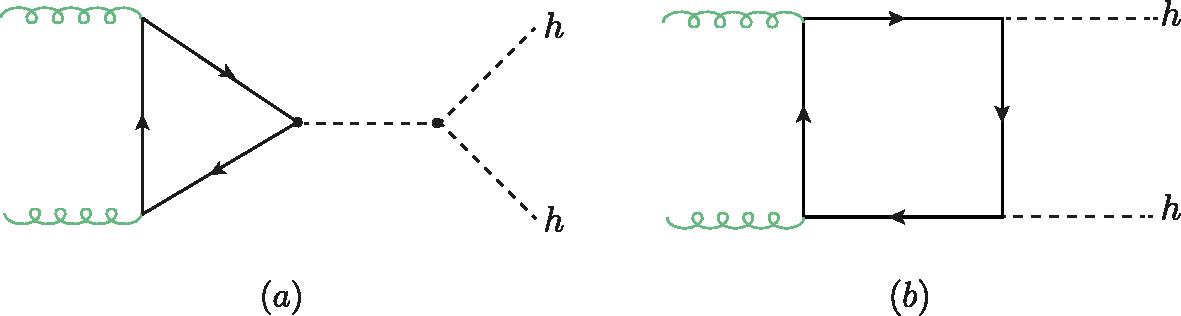
\includegraphics[width = 0.8\textwidth]{./figures/di-higgs-LO-SM}
	\caption{Feynman diagrams for the ggF process of Higgs pair production in the SM.} 
	\label{dihiggs-gridplot}
\end{figure}
%
%%%%%%%%
Calculation of LO in addition to Higher order corrections to Higgs pair production in EFT, MSSM and composite Higgs models can be found in~\cite{Grober:2010yv,Grober:2015cwa,Grober:2017gut,deFlorian:2017qfk,Buchalla:2018yce}.\\ 
The NNLO correction were used according to the Higgs cross section working group recommended values~\cite{Dittmaier:2012vm,deFlorian:2016spz}:
\begin{equation}
	K = \frac{\sigma_{NNLO}}{\sigma_{LO}}, \;\;\;\;\; K_{14 \mathrm{TeV}} \approx 1.71.
\end{equation}
\subsection{Theoretical uncertainties}
There are four main sources of theoretical uncertainties for Higgs pair production:
\begin{enumerate}
	\item Scale uncertainty: coming form the arbitrariness of scales choice.
	\item PDF uncertainties : coming form the uncertainty in the PDF fitting and model.
	\item $\alpha_s$ running uncertainty: originating from the initial value (i.e. $\alpha_s(M_Z) $).
	\item Top mass renormalisation scheme, which involves $m_t$ appearing in the loop propagators and in the top Yukawa.
\end{enumerate}
The computation of the uncertainties is described in ~\cite{Martin:2009bu, Demartin:2010er}. for PDF and $\alpha_s$ uncertainties.
In order to calculate the scale uncertainties, the cross-section was computed with different $ \mu_R$ and $\mu_F$ values ranging between:
\begin{equation}
	\frac{M_{hh}}{4} \leq \mu_R/\mu_F  \leq \,M_{hh}
\end{equation}
As for the $m_t$ renormalisation uncertainty, one uses the $\MSbar$ running of the top mass formula at N$^3$LO~\cite{Baglio:2020wgt}
\begin{equation}
	\overline{m_t} (m_t^{pole}) =m_t^{pole}\, \left( 1+\frac{4}{3 \pi} \alpha_s(m_t^{pole})+10.9 \frac{\alpha^2_s(m_t^{pole})}{\pi^2} +107.11 \frac{\alpha^3_s(m_t^{pole})}{\pi^3} \right) ^{-3} 
\end{equation}
The total 14 TeV ggF $hh$, cross-section at different orders in computation with its uncertainties are shown in~\autoref{ggf_xsres}, which indicates that the uncertainties are dominated by the $m_t$ renormalisation scheme of $\sim -18\%$ uncertainty in the lower envelope.  This is significant part of the uncertainty budget and needs to be resolved by including N$^3$LO corrections to ggF $hh$, such corrections are available in the  HTL~\cite{Chen:2019lzz,Chen:2019fhs}. 
%
\begin{table}
	\centering
	\begin{tabular}{ccccc}
		\toprule
		& $ \sigma$	[fb] & Scale [fb] & PDF$+\alpha_s$ [fb]& Total [fb] \\
		\midrule
		SM HEFT  (LO)      &  $ 18.10$    &   $-$      & $-$   &  $-$ \\
		SM   running mass (LO)  &  $ 16.96$    &   $ -$   & $-$   &  $-$ \\
		SM    (LO)  &  $ 21.45$    &   $ \,^{+4.29}_{-3.43}$   & $\pm 1.46$   &  $ \,^{+4.53}_{-3.73}$ \\
		SM   (NLO)~\cite{Baglio:2012np}  &  $ 33.89$   &   $ \,^{+6.17}_{-4.98}$   & $ \,^{+2.37}_{-2.01}$   &  $ \,^{+6.61}_{-5.37}$ \\
		SM   (NNLO)~\cite{Grazzini:2018bsd}  &  $36.69$    &    $ \,^{+0.77}_{-1.83}$   & $\pm 1.10$   &  $ \,^{+1.66}_{-6.43}$ {\tiny(incl. $m_t$ uncertainty~\cite{Baglio:2020wgt})} \\
		\bottomrule
	\end{tabular}
	\caption{Gluon fusion~(ggF) Higgs pair production cross-section at 14 TeV with theoretical  uncertainties, the HTL/LME is computed using (SM HEFT), top running mass, LO, NLO and NNLO QCD corrections. The NLO and NNLO results are taken from the references cited in the table. The LO results are computed via a FORTRAN code.}
		\label{ggf_xsres}
\end{table}

\section{Other processes\label{otherhh}  }
Like the single Higgs production at hadron colliders, the production of Higgs pairs has the same subdominant channels VBF, di-Higgsstrahlung $ Vhh$ and associates production of Higgs pair with tops $t\bar hh /t j hh$. Their cross-sections and uncertainties at 14 TeV are shown in the \la{table}, while in~\autoref{dihiggs-all} their cross-sections as a function of the centre-of-mass energy $\sqrt{s}$ is shown~\cite{DiMicco:2019ngk}. 

\subsection{VBF $hh$}
Vector boson fusion $hh$ production has the second largest cross-section after ggF $hh$, which is calculated up to N$^3$LO~\cite{Baglio:2012np,Ling:2014sne,Dreyer:2018qbw} inclusively and differentially at NNLO~\cite{Dreyer:2018rfu}. The dominant diagrams are analigious to the single Higgs VBF, which involve the $W/Z$ bosons exchanged in the $t-$channel. The process has the same topology as the -off shell- single Higgs VBF, with the off-shell Higgs giving two final states ones via the trilinear self-coupling. 
\subsection{Di-Higgsstrahlung}
The associated production of Higgs pair with $W$ and $Z$ bosons has a small cross-section compared to ggF and VBF,  this process is known up to NNLO QCD accuracy, which includes the gluon-fusion component in the full computation~\cite{aglio:2012np,Li:2016nrr,Li:2017lbf}. 
\subsection{Associated Higgs pair production with $t$-quarks}
Sometimes called the di-Higgs bremsstrahlung off top quarks~\cite{DiMicco:2019ngk}, this channel has a steeper dependence on $\sqrt{s}$ than the single Higgs bremsstrahlung $t\bar t h$. One can see, for example, from ~\autoref{dihiggs-all} that its cross-section becomes at  roughly the same  values as the VBF's. Only NLO computations for this channels have been carried out~\cite{Frederix:2014hta}. \\ All of the three channels have a relatively small NLO correction, compared to gluon fusion. Which ranges from 10-30\%. 
\begin{figure}[!htpb]
	\centering
	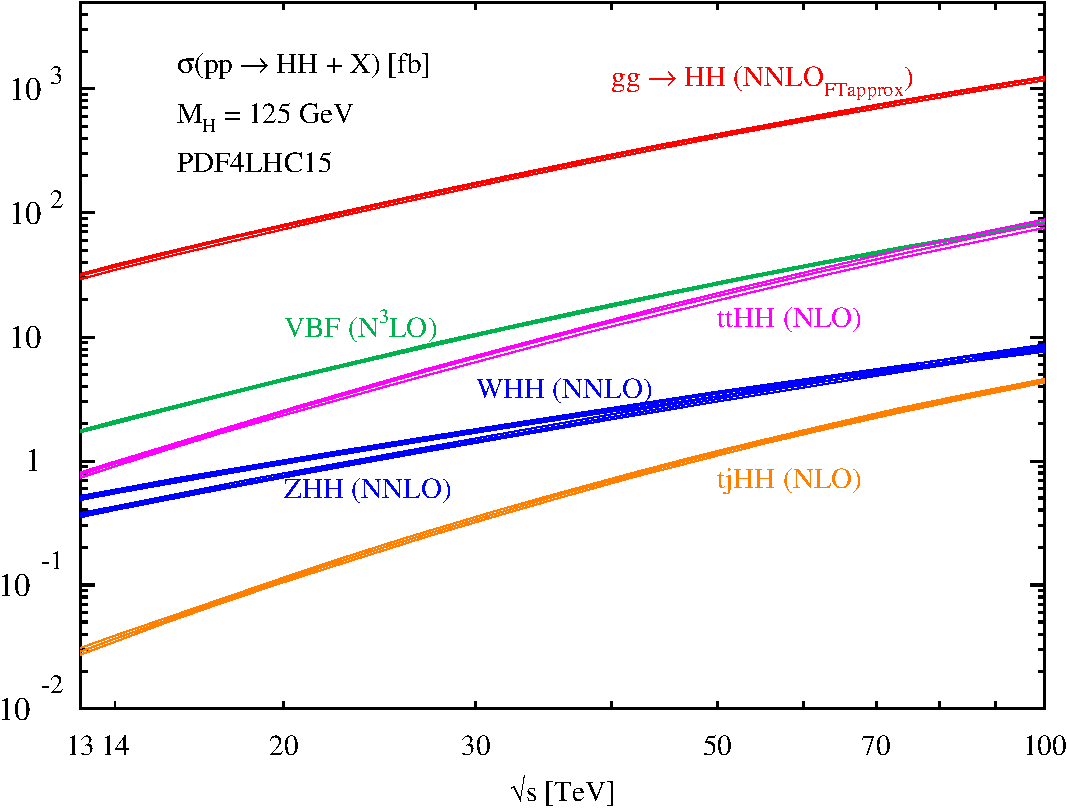
\includegraphics[width = 0.8\textwidth]{./figures/cxn_HH}
	\caption{The cross-section of all di-Higgs processes at the highest available perturbation order as a function of centre-of-mass energy $\sqrt{s}$.The bands show the uncertainties without the top-mass renormalisation scheme. This plot is taken from~\cite{DiMicco:2019ngk}} 
	\label{dihiggs-all}
\end{figure}
%
%%%%%%%%

\section{Experimental overview for Higgs pair production \label{exphh}  }

\section{Summery \label{summtrilinear}  }

%\section{Overview of Light Yukawa searches}
%There are additional measurements of the light-quark Yukawa couplings that might become relevant at HL-LHC or FCC-hh, a careful study of which is beyond the scope of the current work. Yet we attempt to include a discussion here, so as to provide a comparison with our study and to put it into proper context, or to serve as proposal for further studies.
%
%The channel $pp \to h +j $ has been suggested as a probe for charm Yukawa coupling~\cite{Brivio:2015fxa} with charm-tagged jet having a potential bound of $\kappa_c\sim 1$ for the HL-LHC, depending on the charm-tagging scheme. This process could be used for the first and second generations Yukawa couplings by looking at the shapes of kinematic distributions, the most important one being the $p_T$ distribution~\cite{Soreq:2016rae,Bishara:2016jga, Bonner:2016sdg}. The expected HL-LHC 95\% CL bounds are $\kappa_c \in [-0.6,3.0]$, $|\kappa_u |\lesssim 170 $ and $|\kappa_d| \lesssim 990$. The use of $h+j$ process along with other single Higgs processes have also been suggested as indirect probes for Higgs self coupling~\cite{McCullough:2013rea,Gorbahn:2016uoy,Bizon:2016wgr,Degrassi:2016wml,Maltoni:2017ims,Degrassi:2021uik}, due to the contribution of the trilinear coupling to NLO electroweak corrections to these processes. In addition, experimental fits have been carried out for the trilinear coupling from single Higgs observables~\cite{CMS:2018rig,ATLAS:2019pbo}. 
%
%It seems that for the HL-LHC, an optimal bound for the trilinear coupling can be obtained by combing both the data from single-Higgs process as well as Higgs pair production~\cite{DiVita:2017eyz}, with 68\% CL bound on $\kappa_\lambda \in[0.1,2.3]$, compared to the expected bound of $\kappa_\lambda \in [0.0,2.5] \cup [4.9,7.4]$ coming from using di-Higgs measurements alone. Moreover, single Higgs processes, namely $Zh$ and $ W^\pm h$ production, could also be useful in probing charm-Yukawa coupling using a mixture of $b$- and $c$-tagging schemes leveraging the mistagging probability of $c$-jets as $b$-jets in $b$-tagging working points, and vice-versa, in order to break the degeneracy in the signal strength~\cite{Perez:2015lra}. The use of this technique could probe $\kappa_c \sim 1$ in the FCC-hh. Of course, for the charm-Yukawa coupling, the constraints are set to improve significantly, as there has been recent direct observation of $h\to c \bar c$~\cite{ATLAS-CONF-2021-021}. Therefore, from here on, we will mainly concentrate  on the process with more potential for constraining Yukawa couplings of the first generation quarks. 
%
%Rare Higgs decays to mesons, $h \to M +V ,\, \, M = \Upsilon, J/\Psi, \phi\dots$, were also suggested as a probe for light-quark Yukawa couplings~\cite{Bodwin:2013gca,Kagan:2014ila,Konig:2015qat}, and there have been experimental searches for these decays~\cite{ATLAS-CONF-2021-021,CMS:2018gcm} with bounds on the branching ratios, $\mathcal{B} (h \to X, \gamma, \,\,\, X =\Upsilon, J/\Psi,  ) \sim 10^{-4} - 10^{-6}$ at 95\% CL. It was shown in Ref.~\cite{Yu:2017vul}, that the charge asymmetry of the process $pp \to h W^+$ vs $ pp \to h W^-$ can be used as a probe for light-quark Yukawa couplings as well as to break the degeneracy amongst quark flavours. Moreover, the rare process $ pp \to h \gamma$ is also a possible way to distinguish between enhancements of the up- and down-Yukawa couplings~\cite{Aguilar-Saavedra:2020rgo} where the authors have estimated the bounds on the up-Yukawa coupling of $\kappa_u\sim 2000$ at the HL-LHC. Despite some processes appearing more sensitive than others, one should think of these processes as complementary to each other. 
%
%\begin{figure}[t!]
%	%	\centering
%	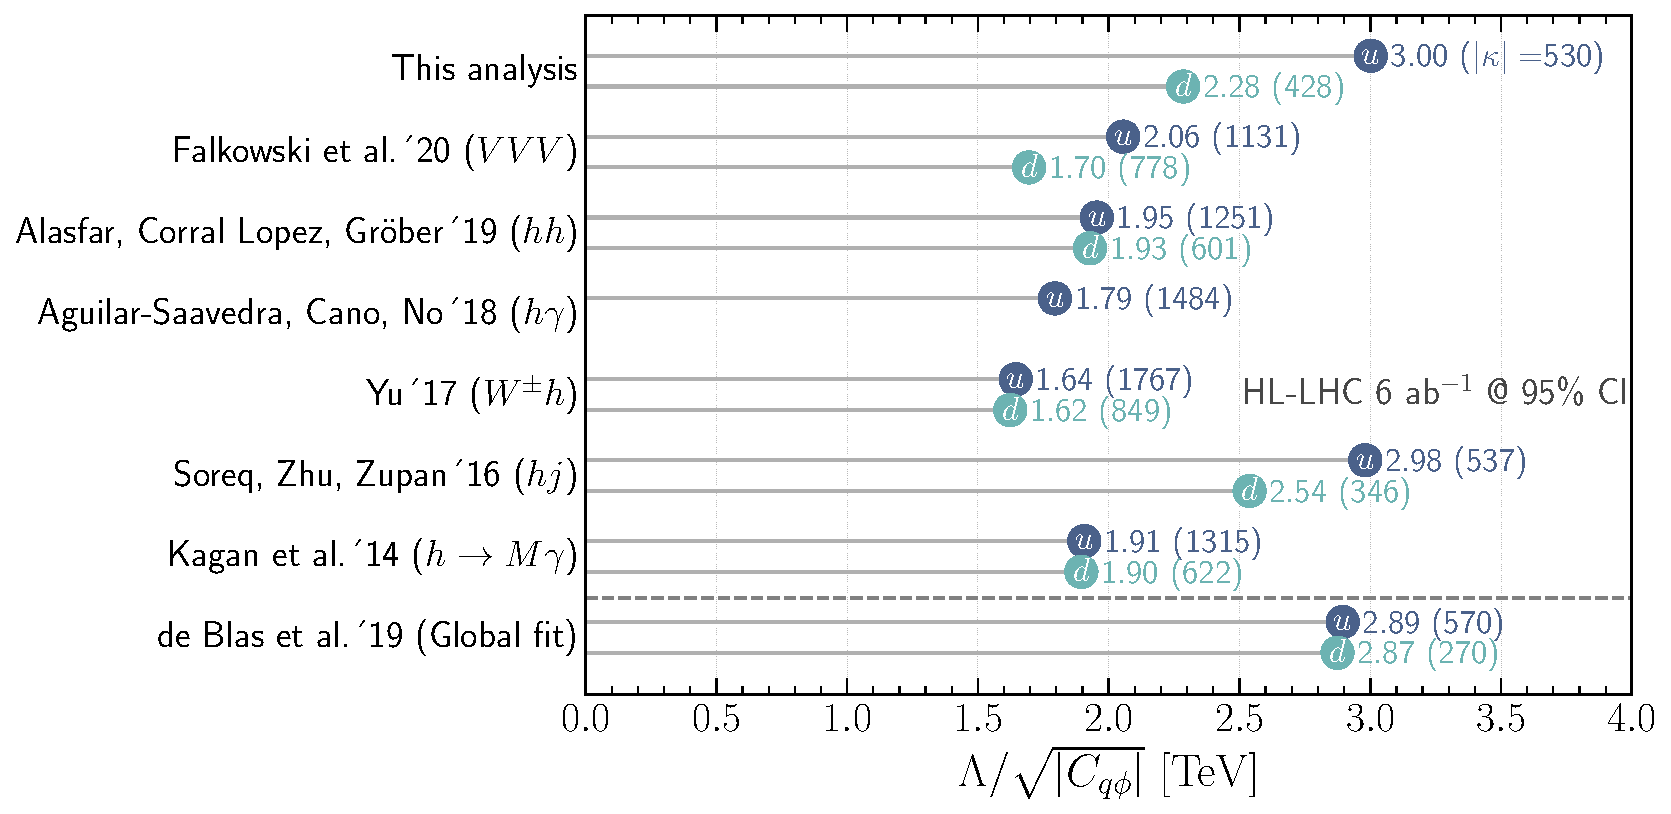
\includegraphics[width=\linewidth]{fig/ueberblick.pdf}
%	\caption{Summary of the $95\%$ CI/CL sensitivity bounds on the SMEFT Wilson coefficients $C_{u\phi}$ (blue), and $C_{d\phi}$ (green). The bounds are interpreted in terms of the NP scale $\Lambda$ that can be reached through the measurements of the Wilson coefficient at the HL-LHC at $6$ \invab, the corresponding $\kappa_q$'s are shown inside the parentheses. Single parameter fit $95\%$ CI bounds are used from this analysis for comparison with previous studies.}
%	\label{fig:comparison}
%\end{figure}
%
%One of the main features of the effective couplings $hh q\bar q$ and $hhh q\bar q$ emerging from SMEFT operator $\mathcal O_{q\phi}$, or the Chiral Lagrangian for that matter, is that these couplings are either free from propagator suppression for $hh q\bar q$ or scale with energy for $hhh q\bar q$ while being safe from strong unitarity constraints. This feature gives processes with multiple Higgs and/or vector bosons $V= W^\pm, Z$ an advantage in constraining $\mathcal O_{q\phi}$. The latter constrains come from the longitudinal degrees of freedom of the gauge bosons  which can be understood from the Goldstone boson equivalence theorem. The use of the final state $VV$ as a probe for $\mathcal O_{q\phi}$ is difficult due to the large SM background. However, the three-boson final state $VVV$ was shown to give strong projected bounds for light-quark Yukawa couplings for HL-LHC with 95\% CL bounds on $\kappa_u \sim 1600$, and $\kappa_d\sim 1100$. A ten fold improvement is expected at FCC-hh~\cite{Falkowski:2020znk} with bounds of order $\kappa_d\sim 30$. 
%Higgs pair production has a smaller SM background compared to $VV$ production, but it has a significantly smaller cross section too, even when compared to $VVV$, as the latter process has already been observed at the LHC~\cite{Sciandra:2688061,CMS-PAS-SMP-19-014}.
%
%On the contrary, Higgs pair production is inaccessible with the runs I-III of the LHC, but it is potentially accessible at the HL-LHC~\cite{Binoth:2006ym} having a $ \sigma \cdot BR\sim 1\mathrm{fb}^{-1}$. However, Higgs pair production, particularly the channel $h \to b \bar b \gamma \gamma $, is of significant interest as it has unique features. The first being the ability to constrain the trilinear and light-quark Yukawa couplings simultaneously, as we show in this work. Secondly, Higgs pair production could probe non-linear relations between Yukawa interaction and $hh q\bar q$ couplings~\cite{Contino:2012xk,Alasfar:2019pmn}. Lastly, Higgs pair production is expected to be significant enhanced in certain models involving modification of light-quark Yukawa couplings (cf. ~\cite{Bar-Shalom:2018rjs,Bauer:2017cov,Egana-Ugrinovic:2021uew})
%
%For future colliders, like the FCC-hh at $100$ TeV, in addition to Higgs pair production triple Higgs production might be an interesting channel for constraining the operators with Wilson coefficient $C_{u\phi}$ and $C_{d\phi}$ due to the energy increase of a Feynman diagram coupling the quarks to three Higgs bosons.   In this case, a similar study to ours should be performed to see whether also in this case it will be important to do a combined fit on the light quark Yukawa couplings together with the trilinear and quartic Higgs self-couplings.\footnote{In~\cite{Papaefstathiou:2047255}, it was shown that $\sim \mathcal{O}(1)$ bounds on the quartic Higgs self-coupling can be reached at the FCC-hh.}
%
%Finally, we note that there are also non collider signatures for enhanced light-quark Yukawa couplings, manifesting in frequency shifts in atomic clocks from Higgs forces at the atomic level~\cite{Delaunay:2016brc}. 